\externaldocument{desenvolvimento}
\chapter{METODOLOGIA}
\label{c.metodologia}

\section{Métodos e Planejamento}
\label{s.metodoseplan}

Planeja-se dividir o estudo de acordo com as seguintes etapas:

\begin{itemize}
	\item[-] Levantamento bibliográfico
	\item[-] Análise e desenvolvimento das técnicas de detecção baseadas em assinatura utilizadas atualmente
	\item[-] Implementação Computacional
	\item[-] Análise dos resultados e conclusão da monografia.
\end{itemize}
A confecção da monografia vai ocorrer juntamente com o andamento das demais
etapas definidas durante toda a extensão do projeto. A ideia é utilizar
máquinas virtuais e emuladores para implementar em caráter de teste os
algoritmos de detecção baseados em assinatura sobre um conjunto de programas
contendo alguns programas já infectados com amostras de \textit{malware} diversas para
observar, em termos gerais, a eficiência do tempo de execução dos algoritmos e
suas respectivas taxas de sucesso. O ambiente pode ser montado em qualquer
máquina que suporte a plataforma Windows e emulador Android, então não há
necessidade de que se reserve material da UNESP para uso exclusivo do projeto.
A figura a seguir ilustra o planejamento do projeto.
\begin{figure}[H]
\caption{\small Estrutura do projeto}
\centering
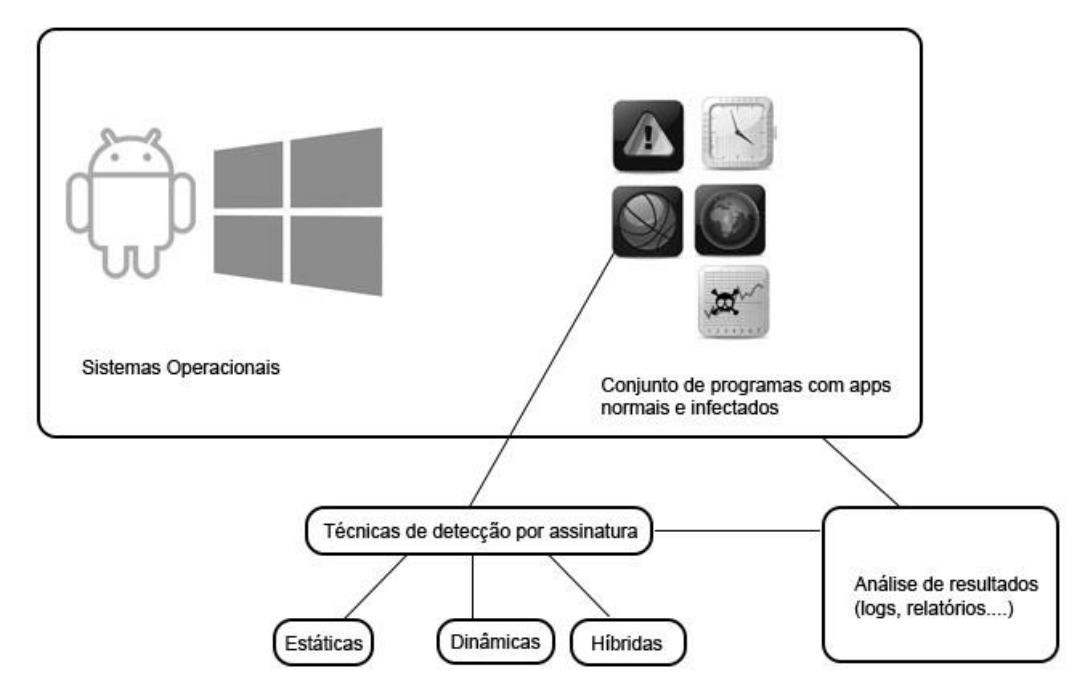
\includegraphics[scale=0.4]{figs/fig2}
\label{f.estrutura_projeto}
\legend{\small Fonte: Elaborada pelo autor.(2016)}
\end{figure}

\section{Materiais Utilizados}
\label{l.material}

\subsection{Servidor Local} % (fold)
\label{sub:servidor}

Foi utilizada uma máquina com 4GB de RAM, 1TB de armazenamento e sistema operacional Windows 10 de arquitetura 64 bits.

\subsection{Yara}
\label{sub:Yara}

Yara é uma ferramenta de código aberto recentemente desenvolvida, cujo intuito é auxiliar desenvolvedores a identificar e classificar amostras de \textit{malware}. Ele é construído em C, porém, com o auxílio de algumas bibliotecas, há a possibilidade de incorporá-lo em scripts de outras linguagens, como Python.Segundo ALVAREZ (2014), O funcionamento do Yara consiste em comparar regras criadas pelo desenvolvedor que descrevem famílias de \textit{malware}, com o código de executáveis quaisquer, ou também de arquivos comprimidos em alguns formatos comuns. As regras podem variar bastante em nível de complexidade e mapearem diversas características do comportamento dos executáveis, que serão detalhadas posteriormente. O projeto no momento encontra-se bastante popular e o programa está sendo utilizado como ferramenta de construção de assinatura de \textit{malware} por desenvolvedores de diversos grupos importantes no ramo, como:
\begin{itemize}
	\item[-] ActiveCanopy
	\item[-] Adlice
	\item[-] CrowdStrike FMS
	\item[-] Fox-IT
	\item[-] Heroku
	\item[-] Kaspersky Lab
	\item[-] Picus Security
	\item[-] ReversingLabs
	\item[-] Symantec
	\item[-] ThreatStream, Inc.
	\item[-] Trend Micro
	\item[-] VirusTotal Intelligence
	\item[-] We Watch Your Website
\end{itemize}

O Yara será utilizado no presente trabalho de conclusão de curso como meio de
aplicação dos algoritmos de assinatura nos programas que serão examinados. Com
o auxílio de scripts desenvolvidos em Python, simularemos uma varredura nesse
conjunto de programas aplicando regras obtidas através de sites como o
\href{yararules.org}{Yara Rules} e o
\href{http://sanesecurity.com/usage/signatures/}{Sane Security}, que
disponibilizam sem custo algum assinaturas de milhões de códigos maliciosos já
capturados pela web. Com esse grande arsenal de assinaturas de \textit{malware}, é
possível testarmos com certa completude as técnicas e assinaturas que são
desenvolvidas no mercado e utilizadas nos sistemas de detecção de intrusão.

\subsubsection{Regras de detecção do Yara}
\label{l.regrasdyara}
O Yara funciona interpretando arquivos que contém características que possivelmente
apontam para o padrão dos elementos da família do \textit{malware} que deve ser
isolado. As regras são escritas com uma sintaxe simples que remete à
construção de uma estrutura de dados em C, contendo strings a serem comparadas
tanto em formato texto quanto hexadecimal, conjuntos de strings, endereços da
memória que ficarão sob monitoramento, limitações de tamanho de arquivo,
expressões regulares, pontos de entrada de execução e variáveis externas.
Todos esses dados do arquivo examinado podem ativar condições, listadas na
construção dessas regras, que vão determinar se o arquivo corresponde ou não à
família definida nas regras de detecção. Para exemplificar mais claramente a
construção e o funcionamento das regras, seguem alguns exemplos de código
obtido do repositório do projeto \href{yararules.org}{Yara Rules} no
\href{github.com}{Github}.

\begin{figure}[h]
	\centering
	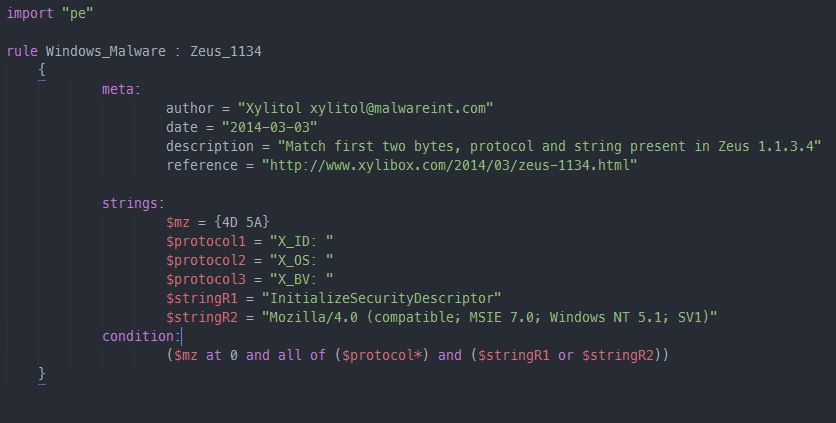
\includegraphics[width=0.95\textwidth]{figs/zeus}
	\caption{Regra de detecção para o \textit{malware} ``Zeus''. Imagem elaborada pelo autor}
	\label{f.regrazeus}
\end{figure}

Na imagem acima temos exemplo de uma descrição para o \textit{malware} chamado ``Zeus''
(também conhecido como ``RPG'', ``ZBot'', ``Infostealer'', entre outros), que é membro da
família dos \textit{Trojans}. Segundo informações da \href{www.wiki-security.com}{Wiki Security}\citeyear{wikisecurity} os danos causados por ele incluem roubo de informações pessoais como senhas de email e de bancos, para posteriormente efetuarem-se transferências para ``contas-mula'' que lavariam o dinheiro das vítimas até
que ele chegasse aos atacantes. O \textit{malware} foi escrito majoritariamente em C
com alguns pequenos trechos em php, e seu código fonte, vazado em 2011, pode
ser encontrado neste outro repositório público do \href{https://github.com/Visgean/Zeus}{Github}.
Como podemos observar, a regra escrita para marcar o trojan verifica os dois primeiros \textit{bytes}, \textit{strings} e o protocolo utilizados por uma determinada versão do ``Zeus'' e fica ativa quando a primeira e uma das outras duas condições são satisfeitas.

Outro exemplo de regra de detecção envolvendo parâmetros semelhantes aos anteriores é a que descreve o \textit{malware} ``Lenovo Superfish''\citeyear{lenovosuperfish}; na verdade esse é o nome de um serviço que vinha embutido em algumas séries de equipamentos lançados pela fabricante Lenovo entre 2014 e 2015, cuja meta era ajudar consumidores a encontrar produtos similares aos que eles buscavam pela web. Esse serviço possuía uma vulnerabilidade de protocolos que foi explorada na criação do \textit{malware} homônimo. No caso, as características que estão sendo mapeadas são novamente os dois primeiros \textit{bytes} do programa, porém com strings em formato e encodificações diferentes das encontradas na regra anterior, como segue na figura:

\begin{figure}[h]
	\centering
	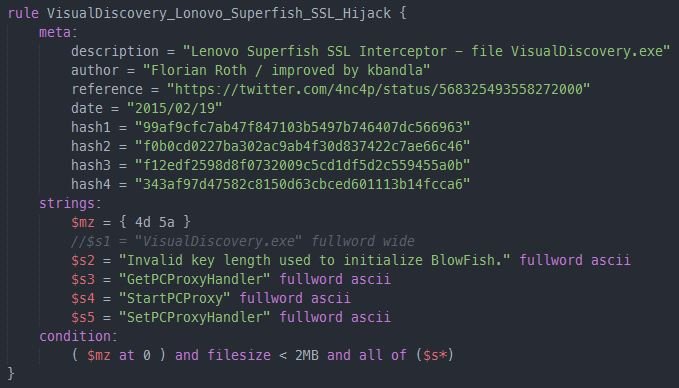
\includegraphics[width=0.95\textwidth]{figs/superfish}
	\caption{Regra de detecção do ``Superfish''}
	\label{f.superfish}
\end{figure}

As regras que utilizaremos no decorrer do projeto serão unificadas num arquivo de índice, compiladas via um\textit{script} em Python para a interpretação do Yara e combinadas com o conjunto completo de arquivos de uma só vez.

\subsection{\textit{Logs} de resultados do Yara} % (fold)
\label{sub:logs_de_resultados_do_yara}

As varreduras efetuadas pelo Yara podem ter seus resultados gravados em arquivos de texto para análise posterior, que podem também definirem-se como \textit{logs}, que por sua vez retornam um dicionário de strings com o seguinte formato:

\begin{lstlisting}[caption=Conteúdo dos arquivos de resultado de varredura, label=resultyara]
{
'tags': ['mal', 'ware'],
'matches': True,
'namespace': 'default',
'rule': 'regras_compiladas',
'meta': {},
'strings': [(81L, '$a', 'abc'), (141L, '$b', 'def')]
}
\end{lstlisting}

O que cada parâmetro significa:
\begin{itemize}
	\item '\textit{tags}': conjunto dos nomes dos programas maliciosos que estão sendo buscados

	\item '\textit{matches}': True significa positivo para infecção

	\item '\textit{rule}': Arquivo com as regras compiladas para aplicação

	\item '\textit{meta}': metadados do arquivo

	\item '\textit{strings}': conjunto de strings para comparação dentro do objeto de varredura
\end{itemize}

\subsection{Python}
\label{sub:python}

É uma linguagem de programação cujo desenvolvimento ocorre desde 1989. No ano
de 1994, foi lançada a primeira distribuição da versão 1.0 oficial da
linguagem e sua versão mais recente foi lançada em setembro de 2015. Para as
necessidades do presente projeto, utilizaremos a versão 2.7 da linguagem, por
suportar a implementação dos \textit{scripts} do Yara e também ser a distribuição mais
estável da linguagem, segundo o \href{www.python.org}{\textit{site} oficial}. O Yara suporta integração com scripts feitos tanto em código C puro como em Python, porém a escolha da linguagem se deu principalmente pela frequência, onde a grande maioria de scripts já prontos e documentados foi feita em Python. As implementações em C são mais comuns em âmbito corporativo, onde se constroem módulos mais otimizados para uso em varreduras de \textit{malware} numa escala mais elevada e o desempenho torna-se um fator mais significativo na aplicação das regras.

\subsection{Clam AV}
\label{sub:clamav}

O Clam AV é um antivírus de código aberto que possui um sistema muito interessante para a montagem de sua base de dados de assinaturas. O \textit{Community Threat Tracking System} funciona coletando os dados de infecções ocorridas nos sistemas dos usuários e aprimorando suas assinaturas automaticamente com base nos dados estatísticos que a comunidade fornece. As bases buscam evidenciar quais \textit{malwares} estão mais ativos no momento, e tornam todas as suas descobertas públicas. Os usuários têm a opção de enviarem dados tanto anonimamente, quanto com um identificador único para cada instalação, e tais dados não são comercializados com terceiros, ou monetizados de alguma outra forma, todas as análises feitas por eles são apenas um serviço gratuito prestado à comunidade \textit{open source}.
No projeto que foi desenvolvido, utilizaram-se bases de dados com assinaturas utilizadas pelo Clam AV em suas próprias varreduras em \textit{scripts} que as descomprimem e convertem para regras do Yara, que por sua vez podem ser editadas ou testadas isoladamente a critério do desenvolvedor.


\subsection{Resumo da metodologia do projeto}
\label{ss.resumo}

O fluxo de desenvolvimento do projeto consiste na aplicação de um índice de regras de detecção do Yara, construído a partir da conversão de arquivos contendo bases de assinaturas do Clam AV para arquivos contendo regras de detecção do Yara, sobre o conjunto de amostras vivas de \textit{malware} obtidas nos repositórios citados na seção do desenvolvimento do projeto. As varreduras são feitas via linha de comando e para agilizá-las, além do uso de índices para agrupar regras, também pode-se automatizar as varreduras em grupos maiores de arquivos aplicando um pouco de \textit{shell script}. Os resultados das varreduras serão armazenados em arquivos de texto que irão conter todos os atributos analisados a cada arquivo a respeito de uma determinada regra. Vamos explicar com um pouco mais de detalhe como ficam caracterizadas as infecções nos \textit{logs} de resultados, com casos de teste envolvendo expectativas de resultados positivos, falso-positivos e negativos. Ao final da seção de desenvolvimento, também será explicada a ideia da aplicação \textit{web} para varreduras remotas e manipulação de regras do Yara.
